\documentclass[12pt, a4paper]{article}

% ─── ENCODING & LANGUAGE ──────────────────────────────────────────
\usepackage[utf8]{inputenc}
\usepackage[T1]{fontenc}
\usepackage[brazilian]{babel}
\usepackage[autostyle]{csquotes}   % aspas corretas em pt-BR

% ─── TYPOGRAPHY ───────────────────────────────────────────────────
\usepackage{mathpazo}              % Palatino — fonte padrão artigos econ
\usepackage[scaled=0.95]{helvet}   % Helvetica para sans (notas de rodapé)
\usepackage{microtype}
\usepackage{indentfirst}           % parágrafo inicial também indentado (ABNT)

% ─── MATH ─────────────────────────────────────────────────────────
\usepackage{amsmath, amssymb, amsthm}
\usepackage{mathtools}
\allowdisplaybreaks                % permite quebra de equações entre páginas

% ─── LAYOUT ───────────────────────────────────────────────────────
% ABNT NBR 14724: margens 3cm (esq/sup) × 2cm (dir/inf) para trabalhos
% Para artigo de disciplina usa-se margem simétrica:
\usepackage[a4paper, left=3cm, right=2.5cm, top=3cm, bottom=2.5cm]{geometry}
\usepackage{setspace}
\setstretch{1.5}                   % espaçamento 1,5 — padrão pós-graduação
\setlength{\parindent}{1.25cm}     % recuo ABNT NBR 14724
\setlength{\parskip}{6pt}

% ─── TABLES & FIGURES ─────────────────────────────────────────────
\usepackage{booktabs}
\usepackage{threeparttable}        % notas de tabela (tnote)
\usepackage{longtable}
\usepackage{graphicx}
\usepackage{caption}
\captionsetup{
  font=small, labelfont=bf, labelsep=period,
  justification=raggedright, singlelinecheck=false
}
\usepackage{subcaption}
\usepackage{float}
\usepackage{multirow}
\usepackage{array}
\newcolumntype{L}[1]{>{\raggedright\arraybackslash}p{#1}}

% ─── BIBLIOGRAPHY ─────────────────────────────────────────────────
\usepackage{natbib}
\bibliographystyle{plainnat}
\setcitestyle{authoryear, round, comma}

% ─── HYPERLINKS ───────────────────────────────────────────────────
\usepackage[
  colorlinks=true, linkcolor=black, citecolor=black,
  urlcolor=black, breaklinks=true,
  pdftitle={Pegada de Acidentes de Trabalho -- MIP-ES 2015},
  pdfauthor={Felipe Carvalho},
  pdfsubject={Economia do Trabalho; Insumo-Produto},
  pdfkeywords={insumo-produto, segurança do trabalho, pegada social, AEAT}
]{hyperref}

% ─── HEADERS & FOOTERS ────────────────────────────────────────────
\usepackage{fancyhdr}
\pagestyle{fancy}
\fancyhf{}
\fancyhead[L]{\small\itshape Pegada de acidentes de trabalho\,\textperiodcentered\,MIP-ES 2015}
\fancyhead[R]{\small\thepage}
\fancyfoot[C]{\small PPGEco/UFES --- PECO-5054/6054 --- 2026/1}
\renewcommand{\headrulewidth}{0.4pt}
\renewcommand{\footrulewidth}{0.4pt}
\setlength{\headheight}{14.5pt}

% ─── CUSTOM COMMANDS ──────────────────────────────────────────────
% Nota de tabela fora do float (fallback sem threeparttable)
\newcommand{\tabnote}[1]{\par\smallskip\footnotesize\textit{Notas:} #1}
% Abreviações comuns
\newcommand{\vbp}{\textsc{vbp}}
\newcommand{\cat}{\textsc{cat}}
\newcommand{\mipes}{\textsc{mip-es}}
\newcommand{\aeat}{\textsc{aeat}}

% ─── TITLE ────────────────────────────────────────────────────────
\title{%
  \large\textsc{Universidade Federal do Espírito Santo}\\
  \small Programa de Pós-Graduação em Economia\\[0.4em]
  \rule{\linewidth}{0.8pt}\\[0.6em]
  \LARGE\bfseries Pegada de Acidentes de Trabalho\\[0.4em]
  \large\normalfont\itshape
    Uma aplicação de insumo-produto estendido à\\
    Matriz Insumo-Produto do Espírito Santo (2015)\\[0.4em]
  \rule{\linewidth}{0.8pt}
}
\author{%
  \large Felipe Carvalho%
  \thanks{Mestrando em Economia, PPGEco/UFES.
          Disciplina PECO-5054/PECO-6054 --- Análise de Insumo-Produto, 2026/1.
          Prof.\ Dr.\ Celso Bissoli Sessa.
          Contato: \href{mailto:fcarva@ppgeco.ufes.br}{\texttt{fcarva@ppgeco.ufes.br}}.}
}
\date{Vitória, maio de 2026}

\begin{document}
\maketitle
\thispagestyle{fancy}
% ── Resumo (pt-BR) ────────────────────────────────────────────────
\renewcommand{\abstractname}{\normalfont\normalsize\bfseries Resumo}
\begin{abstract}
\setstretch{1.0}\small
Este artigo aplica o modelo de Leontief estendido para mensurar a
\textit{pegada de acidentes de trabalho} na economia do Espírito Santo
a partir da Matriz Insumo-Produto estadual de 2015 (35 setores),
usando como vetor satélite os registros oficiais do Anuário Estatístico
de Acidentes do Trabalho (\aeat-2015), que totalizam 12,156~\cat{}s no
estado. Calculando $\mathbf{f}' = \mathbf{a}'\mathbf{L}$ para cada setor,
obtém-se que o componente indireto representa em média 37{,}6\,\% da
pegada total --- indicando que mais de um terço do passivo de acidentes
embutido em qualquer demanda final típica se origina em atividades
distintas das que produzem o bem demandado.
Cruzando intensidade direta ($a_j$) com índices de Rasmussen-Hirschman,
propõe-se uma tipologia de quatro quadrantes que identifica
6~\textit{setores-chave de risco}.
Uma análise de sensibilidade Monte Carlo ($N = 1\,000$, $\sigma_{\log} = 0{,}20$)
confirma que 6~setores permanecem no quadrante crítico em mais de
50\% das iterações. A extração hipotética dos setores petrolífero (0680)
e ferroso (0791) altera a pegada agregada em apenas 2{,}0\%
e 0{,}5\% respectivamente, revelando o
\textit{deslocamento estrutural duplo} do risco ocupacional na economia
capixaba. Um exercício comparativo com a MIP-Brasil 2015 (IBGE, 67~atividades)
mostra ainda que a maior intensidade agregada do ES ($+21\,\%$ vs Brasil)
\textit{não} se explica por efeito-composição (especialização extrativa),
mas por efeito-intensidade nos setores de transformação e serviços ---
exatamente os \textit{propagadores estruturais} identificados pela
tipologia.

\smallskip
\noindent\textbf{Palavras-chave:} insumo-produto; segurança do trabalho;
pegada social; ligações de Rasmussen-Hirschman; Espírito Santo; \aeat-2015.\\
\noindent\textbf{Códigos JEL:} D57; J28; R15.
\end{abstract}

% ── Abstract (EN) ─────────────────────────────────────────────────
\renewcommand{\abstractname}{\normalfont\normalsize\bfseries Abstract}
\begin{abstract}
\setstretch{1.0}\small
This paper applies the extended Leontief model to measure the
\textit{work accident footprint} of the Espírito Santo economy using
the 2015 state input-output matrix (35 sectors) and an official
satellite vector constructed from the 2015 Work Accident Statistical
Yearbook (\aeat-2015), totalling 12,156 registered accidents.
The structural (indirect) component accounts for 37{,}6\,\% of
the total footprint on average, indicating that over one-third of the
accident liability embedded in any unit of final demand originates
in sectors other than the direct producer.
We propose a four-quadrant typology combining accident intensity with
Rasmussen-Hirschman backward linkages, identifying 6~\textit{key
risk sectors}. Monte Carlo sensitivity analysis ($N=1\,000$) confirms
robustness of 6~sectors. Hypothetical extraction of the
oil-and-gas (0680) and iron-ore (0791) sectors changes the aggregate
footprint by 2{,}0\% and 0{,}5\%
respectively, supporting the \textit{double structural displacement}
hypothesis. A comparative exercise against the 2015 Brazilian
input-output matrix (IBGE, 67~activities) shows that the higher
aggregate intensity in ES ($+21\,\%$ vs Brazil) is driven by an
intensity effect, not a composition effect: the state's extractive
specialization, weighted by national intensities, would yield a
\textit{lower} accident rate, contradicting the standard narrative.

\smallskip
\noindent\textbf{Keywords:} input-output; occupational safety; social footprint;
Rasmussen-Hirschman linkages; Espírito Santo; AEAT-2015.\\
\noindent\textbf{JEL Codes:} D57; J28; R15.
\end{abstract}

\vspace{1em}
\noindent\rule{\linewidth}{0.4pt}
\vspace{0.5em}
\setstretch{1.5}

% ════════════════════════════════════════════════════════════════
\section{Introdução}
% ════════════════════════════════════════════════════════════════

A análise da segurança e saúde no trabalho (SST) na economia brasileira
é tradicionalmente conduzida em registro setorial isolado: examinam-se
taxas de incidência por classe da CNAE, a eficácia de Normas
Regulamentadoras específicas, ou correlações entre regulação e
ocorrência~\citep{shimizu2021accident,chagas2011saude,ipea2018terc}.
Falta, com poucas exceções na literatura nacional, um tratamento
\textit{estrutural} do problema --- capaz de mapear como o risco
ocupacional gerado em um setor é transmitido para outros setores via
encadeamentos produtivos até alcançar o consumidor final.

A pergunta é especialmente relevante em economias com especialização
produtiva concentrada em atividades de alto risco. O Espírito Santo é
o caso paradigmático no Brasil contemporâneo: em 2015, os setores de
extração de petróleo e gás (CNAE-IBGE 0680) e extração de minério de
ferro (0791) responderam, somados, por aproximadamente
\textbf{R\$~33,3~bilhões em valor bruto da produção (VBP)} ---
parte de um total extrativo de R\$~34,6~bi (17,5\,\% do VBP estadual
de R\$~198,3~bi).\footnote{Cálculo a partir da MIP-ES 2015 oficial
(IJSN), conforme Seção~\ref{sec:dados}.}
Trata-se de atividades com taxas de acidente persistentemente acima
da média nacional que, simultaneamente, produzem bens com alta
inserção exportadora.

Em nível nacional, o Brasil registrou em 2015 aproximadamente
517~mil acidentes do trabalho com CAT computada no AEAT, ante
12.156~CATs no Espírito Santo \citep{aeat2016}. Em termos de pegada
direta por unidade de produção (CATs por R\$~milhão de VBP), a
intensidade agregada estadual é cerca de 21\,\% superior à média
brasileira (0{,}061 vs 0{,}051 CATs/R\$~M). A Seção~\ref{sec:comparativo}
mostra, contudo, que esse diferencial \textit{não} se explica
pela especialização extrativa do estado --- a decomposição shift-share
revela efeito-composição \textit{negativo} ($-23\,\%$ da diferença) e
efeito-intensidade fortemente \textit{positivo} (+318\,\%), em uma
estrutura econômica em que o ES detém a segunda maior razão
produção-exportações entre os estados brasileiros
\citep{haddad2017iioas}. A abordagem insumo-produto torna possível
separar efeito de especialização setorial, efeito de intensidade e
efeito de estrutura de encadeamentos.

A pergunta deste artigo é, portanto: \textbf{qual o conteúdo de
acidentes de trabalho embutido em uma unidade de demanda final por
setor na economia capixaba, e como a estrutura produtiva redistribui
esse passivo entre quem produz fisicamente o risco e quem o demanda
via produto final?}

A contribuição é dupla. Metodologicamente, transpõe-se para o caso
brasileiro o instrumental de pegadas sociais (\textit{social footprint
analysis}), consolidado na literatura internacional para emissões de
carbono mas aplicado de forma incipiente a variáveis ocupacionais.
Empiricamente, oferece-se a primeira mensuração, ao nosso conhecimento,
da pegada de acidentes para uma economia subnacional brasileira,
usando a MIP-ES 2015 (35\,$\times$\,35) com vetor satélite construído
diretamente dos registros administrativos oficiais do AEAT-2015.

\paragraph{Dimensão estrutural e normativa.}
A relevância do tema extrapola o caso capixaba. O Brasil registrou,
em média, mais de 700~mil acidentes de trabalho anuais notificados no
período 2010--2019 --- o que o torna uma das maiores economias do mundo
em volume absoluto de acidentes ocupacionais~\citep{chagas2011saude}.
Contudo, esse número subestima dramaticamente a realidade: a literatura
estima taxas de subnotificação de cerca de 19\% a nível agregado
nacional~\citep{inss2022subnotificacao} e de 50--70\% em setores com
alta informalidade como construção, agropecuária e serviços
domésticos~\citep{wunsch2004perfil,cordeiro2005underreporting}.
Em uma economia exportadora de commodities como o Brasil --- e,
em particular, o Espírito Santo --- a estrutura produtiva concentra
fisicamente o risco nas atividades de extração e processamento,
enquanto o benefício econômico é exportado. Essa assimetria é, ao
mesmo tempo, estrutural e normativa.

O problema da subnotificação não é ruído aleatório: é estruturalmente
correlacionado com as dimensões de vulnerabilidade que mais importam
para a análise --- setor produtivo, grau de informalidade, forma de
inserção no mercado de trabalho. \citet{hitzig2020normative} denomina
essa situação \textit{lacuna normativa} (\textit{normative gap}): a
distância entre o que um sistema de mensuração foi desenhado para medir
e o que o objetivo normativo da política pública exige que seja medido.
No caso da CAT brasileira, o sistema foi desenhado para o universo de
trabalhadores formais cobertos pelo RGPS; o objetivo normativo da
Segurança e Saúde no Trabalho (SST) abrange a totalidade dos
trabalhadores expostos ao risco. Essa lacuna é institucional,
não acidental --- e tem implicações diretas para qualquer mensuração
estrutural de acidentes via modelo insumo-produto.

\paragraph{Originalidade.}
Esta é a primeira aplicação de análise de pegada social voltada
especificamente à variável \textit{acidentes de trabalho} em uma matriz
insumo-produto subnacional brasileira. As aplicações de IO estendido
para variáveis sociais no Brasil concentram-se em emprego, remuneração
e desigualdade de gênero --- a dimensão de risco ocupacional permanece
um espaço analítico em aberto, apesar da relevância empírica do fenômeno
e da maturidade do instrumental.

O artigo está organizado em nove seções. A Seção~\ref{sec:teorico}
apresenta o referencial teórico. A Seção~\ref{sec:dados} detalha dados
e método. A Seção~\ref{sec:resultados} reporta os resultados empíricos,
incluindo pegada total, tipologia de quadrantes, multiplicadores de
emprego e análise de sensibilidade. A Seção~\ref{sec:hem} apresenta o
Método de Extração Hipotética para todos os 35 setores.
A Seção~\ref{sec:comparativo} posiciona os resultados no contexto
nacional com uma comparação sistemática ES $\times$ Brasil.
A Seção~\ref{sec:discussao} discute o padrão de deslocamento estrutural
duplo. As Seções~\ref{sec:limitacoes} e~\ref{sec:conclusao} discutem
limitações e considerações finais.

% ════════════════════════════════════════════════════════════════
\section{Referencial teórico}
\label{sec:teorico}
% ════════════════════════════════════════════════════════════════

\subsection{O modelo de Leontief estendido}

O modelo aberto de Leontief estabelece que, para uma economia com $n$
setores, o vetor de produção bruta $\mathbf{x}$ relaciona-se ao vetor de
demanda final $\mathbf{y}$ pela identidade fundamental
%
\begin{equation}
\mathbf{x} = (\mathbf{I} - \mathbf{A})^{-1}\, \mathbf{y} = \mathbf{L}\, \mathbf{y},
\label{eq:leontief}
\end{equation}
%
onde $\mathbf{A}$ é a matriz $n \times n$ de coeficientes técnicos
diretos, com $a_{ij} = z_{ij}/x_j$, e
$\mathbf{L} = (\mathbf{I}-\mathbf{A})^{-1}$ é a inversa de Leontief
\citep[cap.~2]{millerblair2009}.

O modelo torna-se \textit{estendido} quando se associa a $\mathbf{L}$
um vetor $\mathbf{a}$ de coeficientes diretos de uma variável satélite.
Definindo
%
\begin{equation}
a_j = \frac{e_j}{x_j},
\label{eq:coeficiente}
\end{equation}
%
em que $e_j$ é o número de CATs no setor $j$ e $x_j$ é o VBP em
R\$~milhões, o \textbf{vetor de pegada total} é
%
\begin{equation}
\mathbf{f}' = \mathbf{a}'\, \mathbf{L},
\label{eq:pegada}
\end{equation}
%
cuja $j$-ésima coordenada $f_j$ reporta o conteúdo total de acidentes
associado a uma unidade de demanda final por produtos do setor $j$,
considerando todos os encadeamentos a montante \citep[cap.~10]{millerblair2009}.

A decomposição direto-indireto é imediata:
%
\begin{equation}
f_j = \underbrace{a_j}_{\text{efeito direto}}
    + \underbrace{(f_j - a_j)}_{\text{efeito indireto}}.
\label{eq:decomposicao}
\end{equation}

Complementarmente, define-se a intensidade de acidentes por trabalhador
exposto como
%
\begin{equation}
\tilde{a}_j = \frac{e_j}{\ell_j},
\label{eq:atilde}
\end{equation}
%
onde $\ell_j$ é o número de ocupações no setor $j$ (RAIS-2015). A
comparação entre $a_j$ e $\tilde{a}_j$ permite separar setores com alta
pegada por VBP (geralmente labor-intensivos com baixo salário) de setores
com alta taxa de acidente por trabalhador (periculosidade intrínseca).

\subsection{Pegadas sociais}

A literatura de \textit{footprint analysis} nasceu como extensão direta
da contribuição pioneira de \citet{leontief1970}. \citet{hoekstra2002virtual}
consolidam a pegada hídrica e \citet{hertwich2009carbon}, a pegada de
carbono. A extensão para variáveis sociais --- empregos, salários, gênero,
mortes ocupacionais --- teve em \citet{alsamawi2014employment} seu marco
metodológico.

No Brasil, aplicações robustas cobrem variáveis ambientais
\citep{carvalho2009intensidade,souza2016reducing} e sociais
\citep{perobelli2016decomposicao,made2021multiplicadores,guilhotosesso2010estimacao}.
O Centro de Pesquisa em Macroeconomia das Desigualdades
(MADE/FEA-USP) tem avançado na mensuração dos efeitos distributivos
de políticas via modelos IO, com destaque para os multiplicadores de
produto e renda associados a transferências sociais~\citep{made2021multiplicadores}
e à bioeconomia regional~\citep{made2023agroflorestais}.
O NEREUS/USP, por sua vez, fornece a principal plataforma brasileira
de matrizes inter-regionais, permitindo a comparação sistemática entre
estados~\citep{haddad2017iioas,nereus2024mips}.
A dimensão de risco ocupacional, contudo, permanece um espaço
analítico em aberto nessa literatura.
É precisamente nessa lacuna que se insere o presente artigo.

\subsection{Multiplicadores de emprego}

O coeficiente direto de emprego $e_j = \ell_j / x_j$ (trabalhadores
por R\$~milhão de produção) alimenta o multiplicador de emprego Tipo~I
%
\begin{equation}
m^e_j = \mathbf{e}'\, \mathbf{L}_{\cdot j} = \sum_i e_i\, l_{ij},
\label{eq:mult_emprego}
\end{equation}
%
que reporta o número de postos de trabalho gerados direta e
indiretamente para cada R\$~milhão de demanda final do setor $j$.
O multiplicador de emprego contextualiza a pegada de acidentes: um
setor pode ter $f_j$ elevado simplesmente por ser trabalho-intensivo
(e portanto com $\ell_j$ grande), não necessariamente por ser
intrinsecamente perigoso.

\subsection{Ligações de Rasmussen-Hirschman}

Os índices clássicos de ligação \citep{rasmussen1956studies} são
derivados da inversa de Leontief normalizada. O \textit{índice de
ligação para trás} do setor $j$ é
%
\begin{equation}
U_j^B = \frac{\bar{l}_{\cdot j}}{\bar{l}_{\cdot\cdot}},
\label{eq:linkage_back}
\end{equation}
%
onde $\bar{l}_{\cdot j}$ é a média da $j$-ésima coluna de $\mathbf{L}$
e $\bar{l}_{\cdot\cdot}$ é a média geral. $U_j^B > 1$ indica que o setor
demanda insumos acima da média da economia. O \textit{índice de ligação
para frente} $U_j^F$ é calculado analogamente pelas linhas de~$\mathbf{L}$.

A combinação \textbf{alta $a_j$} e \textbf{alto $U_j^B$} caracteriza o
que denominamos \textit{setores-chave de risco}: atividades cuja
periculosidade própria é amplificada pelo seu papel a montante na cadeia.

\subsection{Subnotificação como lacuna normativa}

A categoria analítica central para interpretar as limitações do vetor
satélite deste artigo é a de \textit{lacuna normativa}
(\textit{normative gap}), conforme desenvolvida por
\citet{hitzig2020normative} no campo do design de mecanismos. Uma
lacuna normativa existe quando o critério de desempenho de um mecanismo
diverge sistematicamente do critério normativo que fundamenta sua
existência. No caso dos sistemas de notificação de acidentes de
trabalho, o mecanismo --- a CAT vinculada ao RGPS --- otimiza para a
população de trabalhadores formais com vínculo celetista, enquanto o
objetivo normativo (proteção integral do trabalhador) abrange um
universo substancialmente mais amplo.

A literatura brasileira documenta essa lacuna com precisão crescente.
\citet{chagas2011saude} estimam subnotificação agregada em torno de
19\% para trabalhadores formais, com variação setorial pronunciada.
\citet{wunsch2004perfil} demonstrou que na agropecuária --- setor com
$a_j$ baixo em nosso modelo, mas com $\tilde{a}_j$ provavelmente
elevado --- a subnotificação chega a dois terços dos eventos reais.
\citet{cordeiro2005underreporting} confirmaram padrão semelhante em
municípios de médio porte com base industrial diversificada.

Para a análise de insumo-produto estendido, essa lacuna tem implicações
diretas. O vetor $\mathbf{a}$ construído com dados do AEAT é um piso
\textit{sistematicamente} enviesado, não um piso \textit{aleatório}:
a subnotificação é positivamente correlacionada com informalidade e
negativamente correlacionada com a capacidade institucional de
notificação do setor. A análise Monte Carlo adotada
($\sigma_{\log} = 0{,}20$) trata a incerteza como proporcional e
independente entre setores --- o que é metodologicamente conservador
mas normativamente ingênuo. A subnotificação real é setorialmente
estruturada: setores como saúde privada (8692) e refino (1900) têm
notificação fidedigna; setores como agropecuária (0191) e construção
(4180) provavelmente possuem $a_j$ real substancialmente superior ao
registrado. Essa assimetria comprime artificialmente o diferencial entre
``setores seguros'' e ``setores perigosos'' na tipologia de quadrantes,
ao mesmo tempo que sub-representa o passivo de acidentes dos
trabalhadores mais vulneráveis da economia capixaba.

% ════════════════════════════════════════════════════════════════
\section{Dados e método}
\label{sec:dados}
% ════════════════════════════════════════════════════════════════

\subsection{Matriz insumo-produto}

Utiliza-se a Matriz Insumo-Produto do Espírito Santo de 2015, versão
oficial do Instituto Jones dos Santos Neves (IJSN) em 35 setores
produtivos, valores correntes em R\$~milhões. As matrizes $\mathbf{A}$
e $\mathbf{L}$ são lidas diretamente das Tabelas~11 e~12 do arquivo XLSX
oficial (\textit{Matriz\_Insumo-Produto\_MIP\_35x35.xlsx}), eliminando
erros de transcrição presentes em versões anteriores baseadas em PDF.
A reconstrução é validada por
$\|(\mathbf{I}-\mathbf{A})\mathbf{L} - \mathbf{I}\|_F = 2{,}06 \times 10^{-15}$
(precisão de máquina).

Para a análise do multiplicador de emprego, utiliza-se o vetor de
ocupações formais por setor extraído da RAIS-2015 (Ministério do
Trabalho), compatibilizado com a classificação setorial da MIP-ES via
tabela de tradutores CNAE\,2.0/SCN-IBGE.

\subsection{Vetor satélite de acidentes}

O vetor satélite $\mathbf{a}$ é construído a partir do
\textit{Anuário Estatístico de Acidentes do Trabalho}
\citep{aeat2016}, publicação oficial da Secretaria de Previdência Social.
Utiliza-se o Capítulo~19 do AEAT-2015, que desagrega as Comunicações de
Acidentes de Trabalho (CAT) por classe CNAE\,2.0 e por unidade da
federação. Para cada setor $j$ da MIP-ES calcula-se
%
\begin{equation}
a_j^{\text{ES}} = \frac{\text{CATs}_j^{\,\text{ES, 2015}}}{x_j^{\,\text{ES, 2015}}},
\label{eq:aj}
\end{equation}
%
com $x_j$ em R\$~milhões. A unidade resultante é
``acidentes por R\$~milhão de produção bruta''.
A compatibilização entre CNAE\,2.0 e os setores da MIP-ES segue a
tabela de tradutores oficial do IBGE (92 entradas; cobertura de 100\%
das CNAEs presentes no AEAT para o ES).

\paragraph{Limitações da fonte.}
O AEAT registra apenas acidentes de trabalhadores cobertos pelo RGPS.
Não são capturados servidores estatutários (setores 8400, 8591, 8691),
trabalhadores informais ($\approx 38\%$ da força de trabalho no ES em
2015, PNAD-Contínua 4T/2015) e empregados domésticos sem CAT registrada
(setor 9700). Os resultados devem ser lidos como \textit{estimativa de
piso (lower bound)} da pegada real de acidentes, com direção de
enviesamento monotônica e efeito aproximadamente homotético sobre $a_j$.

\paragraph{Subnotificação heterogênea e suas implicações.}
A magnitude da subnotificação varia entre setores de forma sistemática,
não aleatória. \citet{chagas2011saude} e \citet{wunsch2004perfil}
estimam fator de subnotificação de 50--70\% em setores de alta
informalidade (agropecuária, construção, serviços domésticos), contra
cerca de 19\% para o agregado nacional~\citep{inss2022subnotificacao}.
Essa heterogeneidade setorial tem consequência direta sobre a análise
de quadrantes: setores como agropecuária (0191) e construção civil
(4180) aparecem com $a_j$ baixo não porque são pouco perigosos, mas
porque a subnotificação suprime o numerador. Na linguagem de
\citet{hitzig2020normative}, o mecanismo CAT/RGPS produz uma
\textit{lacuna normativa} que é amplamente setorialmente estruturada.
A análise Monte Carlo com $\sigma_{\log}=0{,}20$ independente entre
setores constitui, portanto, um limite inferior da incerteza real: uma
perturbação metodologicamente mais precisa exigiria covariâncias
positivas entre informalidade setorial e a magnitude do choque em
$a_j$. A robustez a perturbações assimétricas setorialmente estruturadas
permanece como extensão metodológica para trabalho futuro
(Seção~\ref{sec:conclusao}).

\subsection{Exercícios analíticos}

Cinco produtos analíticos compõem os resultados:
%
\begin{enumerate}
  \item \textbf{Pegada total por setor.} Cálculo de
    $\mathbf{f}' = \mathbf{a}'\, \mathbf{L}$ com decomposição
    direto/indireto e razão $f_j/a_j$ (amplificação estrutural).
  \item \textbf{Tipologia de quadrantes.} Plano $(a_j,\, U_j^B)$ com
    cortes pelas médias: \textit{Setor-chave de risco},
    \textit{Propagador estrutural}, \textit{Risco localizado},
    \textit{Residual}.
  \item \textbf{Multiplicador de emprego.} Cálculo de $m^e_j$ e
    $\tilde{a}_j = e_j/\ell_j$ (intensidade por trabalhador exposto).
  \item \textbf{Análise de sensibilidade Monte Carlo.}
    $N=1\,000$ perturbações log-normais em $a_j$
    ($\sigma_{\log}=0{,}20$), avaliando robustez do quadrante e
    intervalos percentis da pegada.
  \item \textbf{Método de Extração Hipotética (HEM).} Para cada um
    dos 35 setores, calcula-se a queda em $\sum f$ resultante de
    zerar simultaneamente linha e coluna de $\mathbf{A}$ e
    componente de $\mathbf{y}$ \citep{dietzenbacher2013expanding}.
\end{enumerate}

  % ════════════════════════════════════════════════════════════════
  \section{Resultados}
  \label{sec:resultados}
  % ════════════════════════════════════════════════════════════════

  \subsection{Pegada total e decomposição}

  O vetor satélite construído a partir do AEAT-2015 soma 12,156~CATs
  registradas no Espírito Santo. A pegada estrutural
  $\mathbf{f}' = \mathbf{a}'\mathbf{L}$ foi calculada para os 35 setores da
  MIP-ES; os 10~maiores valores de~$f_j$ estão na
  Tabela~\ref{tab:top10}.

  A observação central é que o componente indireto representa, em
  média, 37{,}6\,\% da pegada total --- mais de um terço do passivo
  de acidentes embutido em qualquer demanda final típica se origina em
  setores distintos do produtor do bem demandado. A amplificação média
  $f_j/a_j$ é 2{,}09, indicando que cada R\$~milhão de
  demanda final carrega, indiretamente, o dobro dos acidentes da
  atividade que o produz diretamente.

  O setor com maior $f_j$ é \textbf{Saúde privada~(8692)},
  com $f = 0{,}735$~CATs/R\$~M, amplificação
  de 1{,}13 e 11{,}8\,\%
  de componente indireto. Este resultado reflete o caráter
  trabalho-intensivo do setor e sua notificação fidedigna de CATs ---
  o que deve ser contextualizado pela análise de multiplicadores de
  emprego (Seção~\ref{sec:emprego}).

  \begin{table}[H]
  \centering
  \small
  \caption{Top~10 setores por pegada total $f_j$, MIP-ES 2015}
  \label{tab:top10}
  \begin{tabular}{lp{5.2cm}rrrrrr}
  \toprule
  \textbf{Cód.} & \textbf{Setor} & $a_j$ & $f_j$ & $f_j/a_j$ & \%~ind. & $U_j^B$ \\
  \midrule
    8692 & Saúde privada & 0{,}648 & 0{,}735 & 1{,}13 & 11{,}8\,\% & 0{,}948 \\
1900 & Refino de petróleo, coquerias e fabric\ldots & 0{,}320 & 0{,}359 & 1{,}12 & 10{,}9\,\% & 1{,}201 \\
1600 & Fabricação de produtos da madeira, móv\ldots & 0{,}220 & 0{,}255 & 1{,}16 & 13{,}9\,\% & 0{,}981 \\
5280 & Armazenamento, atividades auxiliares d\ldots & 0{,}154 & 0{,}198 & 1{,}28 & 22{,}0\,\% & 1{,}054 \\
2900 & Fabricação de automóveis, caminhões, p\ldots & 0{,}147 & 0{,}187 & 1{,}28 & 21{,}6\,\% & 1{,}037 \\
7800 & Atividades administrativas e serviços\ldots & 0{,}156 & 0{,}174 & 1{,}12 & 10{,}6\,\% & 0{,}875 \\
0280 & Produção florestal; pesca e aquicultur\ldots & 0{,}123 & 0{,}156 & 1{,}27 & 21{,}3\,\% & 1{,}005 \\
9480 & Organizações associativas e outros ser\ldots & 0{,}112 & 0{,}153 & 1{,}37 & 27{,}0\,\% & 1{,}127 \\
2300 & Fabricação de produtos de minerais não\ldots & 0{,}105 & 0{,}148 & 1{,}41 & 28{,}9\,\% & 1{,}098 \\
0580 & Extração de carvão mineral e de minera\ldots & 0{,}109 & 0{,}127 & 1{,}17 & 14{,}7\,\% & 0{,}888 \\
  \bottomrule
  \end{tabular}
  \caption*{\footnotesize $f_j$: CATs/R\$~M de demanda final.
  $a_j$: intensidade direta (CATs/R\$~M VBP).
  $U_j^B$: índice de ligação para trás normalizado.}
  \end{table}

  A Figura~\ref{fig:pegada} apresenta a decomposição visualmente.
  Dois casos polares são instrutivos. O setor com maior componente
  indireto relativo é aquele em que a cadeia a montante carrega risco
  substancialmente acima do produzido diretamente; em contrapartida,
  setores extrativos mostram componente indireto baixo, refletindo
  baixa integração na cadeia produtiva regional.

  \begin{figure}[H]
  \centering
  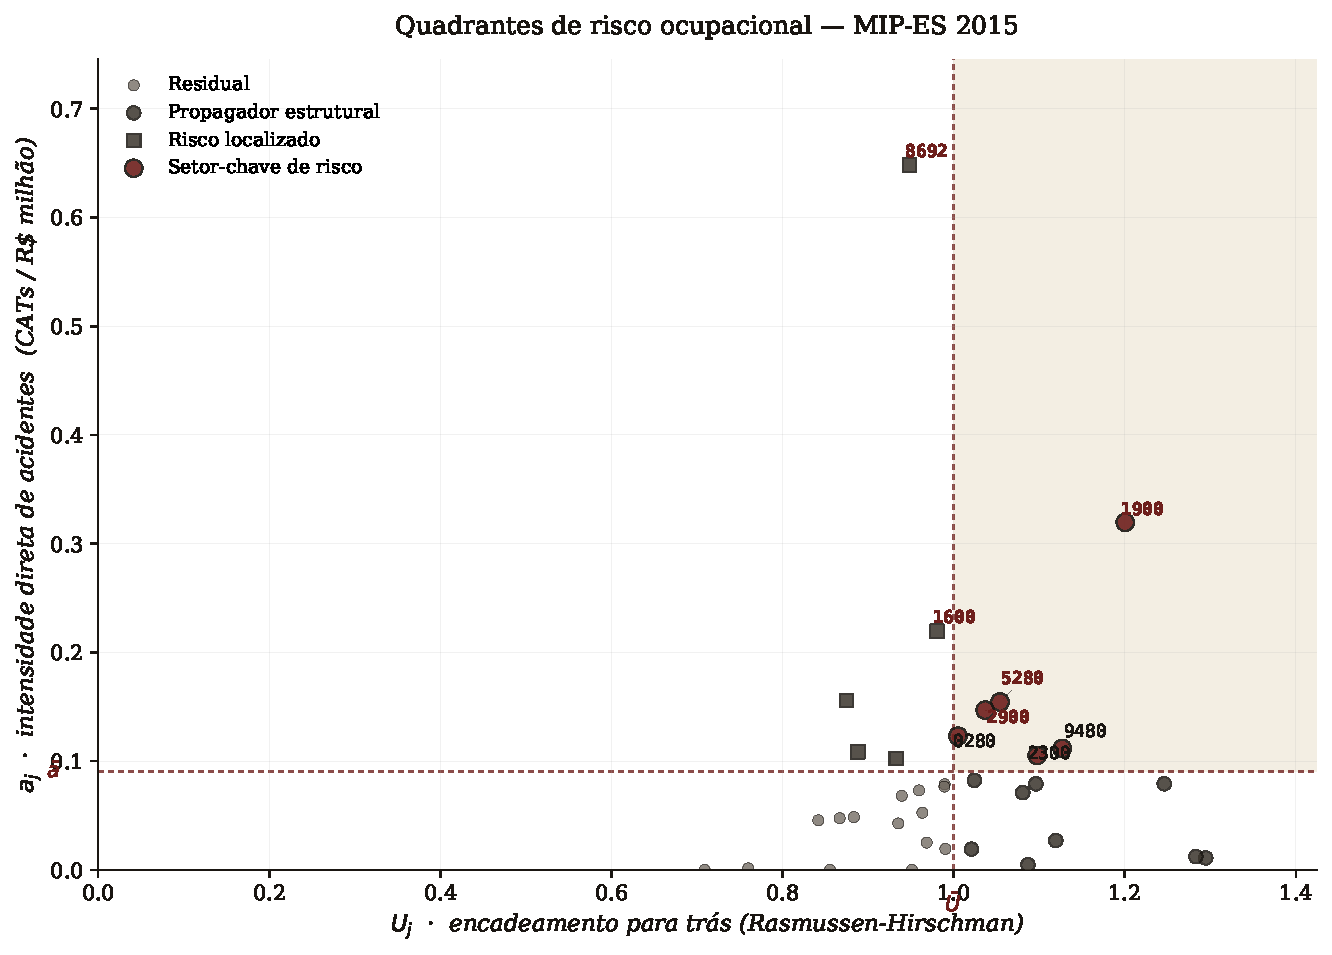
\includegraphics[width=0.95\textwidth]{../outputs/figures/quadrante_risco_es.pdf}
  \caption{Plano $(U_j^B,\, a_j)$ --- tipologia de quadrantes de risco
  (cortes pelas médias $\bar{a} = 0{,}090$ e
  $\bar{U} = 1{,}000$).
  \textbf{Setor-chave de risco}: alta intensidade direta e alto
  encadeamento para trás.
  \textbf{Propagador estrutural}: baixa intensidade mas alto
  encadeamento (transmite risco alheio).
  \textbf{Risco localizado}: alta intensidade mas baixo encadeamento.
  \textbf{Residual}: baixa intensidade e baixo encadeamento.}
  \label{fig:pegada}
  \end{figure}

  \subsection{Tipologia de quadrantes}

  O plano $(a_j, U_j^B)$ com cortes pelas médias
  $\bar{a} = 0{,}090$ e $\bar{U}^B = 1{,}000$
  identifica 6~\textit{setores-chave de risco}
  (Tabela~\ref{tab:chave}) e 9~\textit{propagadores estruturais}
  --- setores que, apesar de baixa intensidade própria, têm alto
  encadeamento para trás e transmitem risco gerado em outras atividades.

  \begin{table}[H]
  \centering
  \small
  \caption{Setores-chave de risco (alta $a_j$ e alto $U_j^B$), MIP-ES 2015}
  \label{tab:chave}
  \begin{tabular}{lp{5.2cm}rrrr}
  \toprule
  \textbf{Cód.} & \textbf{Setor} & $a_j$ & $U_j^B$ & $m^e_j$ & $\tilde{a}_j$ \\
  \midrule
    1900 & Refino de petróleo, coquerias e fabricação de\ldots & 0{,}320 & 1{,}201 & 41{,}85 & 0{,}1082 \\
5280 & Armazenamento, atividades auxiliares dos tran\ldots & 0{,}154 & 1{,}054 & 14{,}13 & 0{,}0189 \\
2900 & Fabricação de automóveis, caminhões, peças e\ldots & 0{,}147 & 1{,}037 & 7{,}49 & 0{,}0395 \\
0280 & Produção florestal; pesca e aquicultura & 0{,}123 & 1{,}005 & 68{,}37 & 0{,}0021 \\
9480 & Organizações associativas e outros serviços p\ldots & 0{,}112 & 1{,}127 & 56{,}70 & 0{,}0023 \\
2300 & Fabricação de produtos de minerais não-metáli\ldots & 0{,}105 & 1{,}098 & 10{,}45 & 0{,}0178 \\
  \bottomrule
  \end{tabular}
  \caption*{\footnotesize $m^e_j$: multiplicador de emprego Tipo~I.
  $\tilde{a}_j$: CATs por trabalhador exposto (RAIS-2015).}
  \end{table}

  \subsection{Multiplicadores de emprego e intensidade por trabalhador}
  \label{sec:emprego}

  Um setor pode ter $a_j$ elevado por dois motivos distintos: (i) é
  genuinamente perigoso (alta taxa de acidente por trabalhador), ou
  (ii) é trabalho-intensivo com VBP por trabalhador baixo. A comparação
  entre $a_j$ e $\tilde{a}_j = e_j/\ell_j$ permite separar esses
  efeitos.

  Os cinco setores com maior multiplicador de emprego $m^e_j$
  (excluindo serviços domésticos) são:

  \begin{table}[H]
  \centering
  \small
  \caption{Top-5 multiplicadores de emprego $m^e_j$, MIP-ES 2015}
  \label{tab:emprego}
  \begin{tabular}{lp{5.2cm}rrrr}
  \toprule
  \textbf{Cód.} & \textbf{Setor} & $m^e_j$ & $a_j$ & $\tilde{a}_j$ & $f_j$ \\
  \midrule
    0191 & Agricultura, inclusive o apoio à agricultura\ldots & 84{,}82 & 0{,}048 & 0{,}0006 & 0{,}066 \\
0280 & Produção florestal; pesca e aquicultura & 68{,}37 & 0{,}123 & 0{,}0021 & 0{,}156 \\
9480 & Organizações associativas e outros serviços p\ldots & 56{,}70 & 0{,}112 & 0{,}0023 & 0{,}153 \\
1900 & Refino de petróleo, coquerias e fabricação de\ldots & 41{,}85 & 0{,}320 & 0{,}1082 & 0{,}359 \\
1300 & Fabricação de produtos têxteis, artefatos do\ldots & 31{,}66 & 0{,}073 & 0{,}0027 & 0{,}098 \\
  \bottomrule
  \end{tabular}
  \caption*{\footnotesize $m^e_j$: trabalhadores gerados (direta e
  indiretamente) por R\$~M de demanda final. $\tilde{a}_j$: CATs por
  trabalhador no setor produtor.}
  \end{table}

  \subsection{Análise de sensibilidade Monte Carlo}

  Para avaliar a robustez dos resultados frente à subnotificação
  heterogênea de CATs, perturbou-se o vetor $\mathbf{a}$ com ruído
  log-normal multiplicativo ($\mu=0$, $\sigma_{\log}=0{,}20$, $N=1\,000$
  iterações, semente 2026). Para cada iteração foram recalculados
  $\mathbf{f}'$ e a classificação de quadrante de cada setor.

  A Tabela~\ref{tab:sensibilidade} reporta os setores que permanecem
  no quadrante \textit{Setor-chave de risco} em mais de 50\% das
  iterações --- 6~setores no total, com coeficiente de
  variação médio de~$f_j$ de 0{,}170.

  \begin{table}[H]
  \centering
  \small
  \caption{Setores robustos --- probabilidade de permanecer em
  \textit{Setor-chave de risco} (Monte Carlo, $N=1\,000$)}
  \label{tab:sensibilidade}
  \begin{tabular}{lp{5.2cm}rrrrr}
  \toprule
  \textbf{Cód.} & \textbf{Setor} & Prob. & $f_{P5}$ & $f_{P50}$ & $f_{P95}$ & CV \\
  \midrule
    1900 & Refino de petróleo, coquerias e fabricação de\ldots & 1{,}00 & 0{,}273 & 0{,}361 & 0{,}484 & 0{,}183 \\
5280 & Armazenamento, atividades auxiliares dos tran\ldots & 0{,}99 & 0{,}153 & 0{,}196 & 0{,}262 & 0{,}167 \\
2900 & Fabricação de automóveis, caminhões, peças e\ldots & 0{,}99 & 0{,}145 & 0{,}189 & 0{,}250 & 0{,}171 \\
0280 & Produção florestal; pesca e aquicultura & 0{,}93 & 0{,}119 & 0{,}155 & 0{,}207 & 0{,}177 \\
9480 & Organizações associativas e outros serviços p\ldots & 0{,}82 & 0{,}121 & 0{,}154 & 0{,}195 & 0{,}151 \\
2300 & Fabricação de produtos de minerais não-metáli\ldots & 0{,}72 & 0{,}113 & 0{,}148 & 0{,}195 & 0{,}169 \\
  \bottomrule
  \end{tabular}
  \caption*{\footnotesize Prob.: fração das iterações em que o setor
  classificou como Setor-chave. $f_{P5/50/95}$: percentis da distribuição
  empírica de $f_j$. CV: coeficiente de variação.}
  \end{table}

  A Figura~\ref{fig:sensibilidade} apresenta o boxplot da distribuição
  de $f_j$ para os 15~setores com maior mediana.

  \begin{figure}[H]
  \centering
  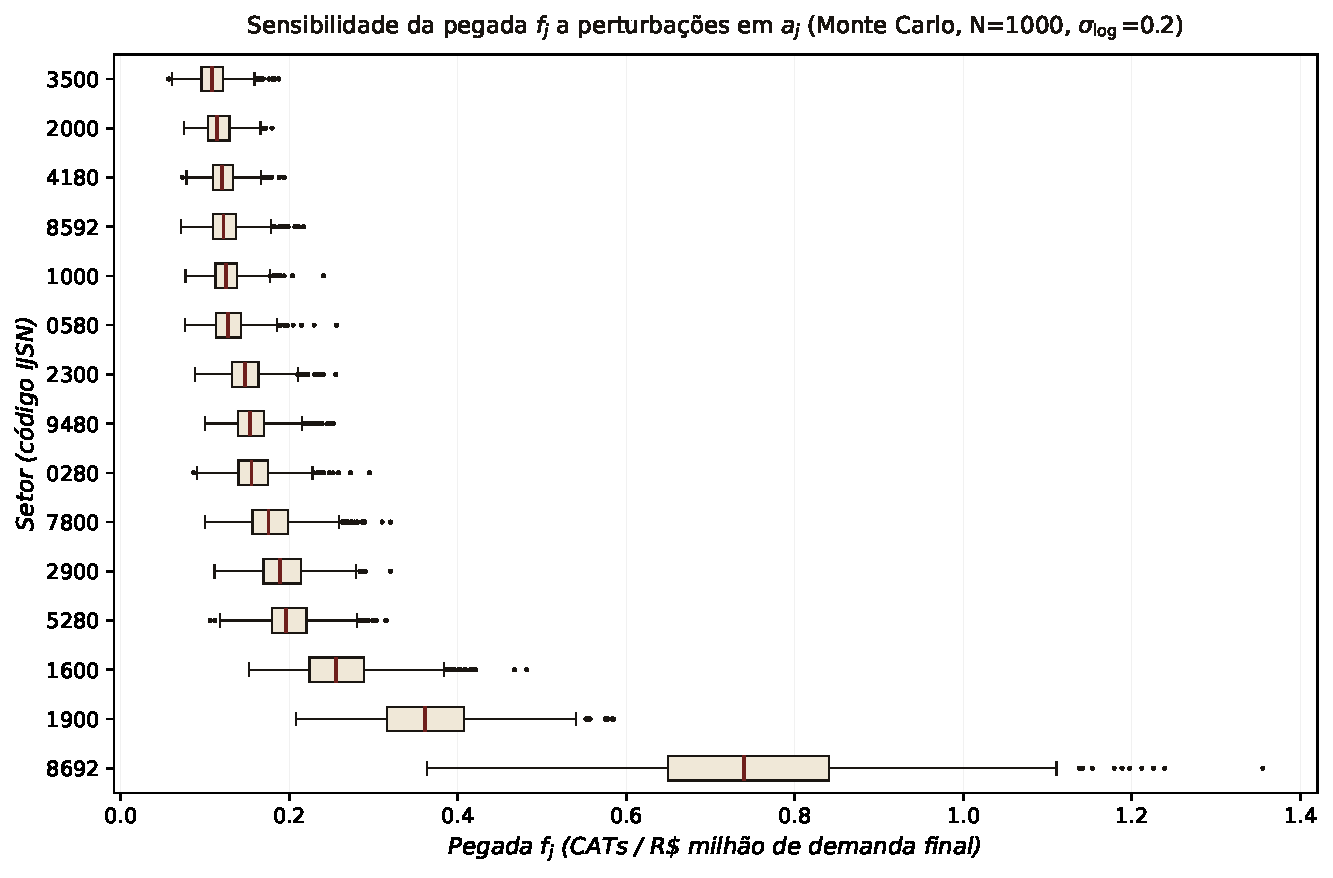
\includegraphics[width=0.92\textwidth]{../outputs/figures/sensibilidade_pegada.pdf}
  \caption{Distribuição de $f_j$ sob perturbação Monte Carlo
  ($N=1\,000$, $\sigma_{\log}=0{,}20$) --- top-15 setores por
  $f$ mediana. Linhas vermelhas: mediana; caixas: IQR; bigodes: $1{,}5 \times \text{IQR}$.}
  \label{fig:sensibilidade}
  \end{figure}

  % ════════════════════════════════════════════════════════════════
  \section{Método de Extração Hipotética}
  \label{sec:hem}
  % ════════════════════════════════════════════════════════════════

  O Método de Extração Hipotética (HEM) de \citet{dietzenbacher2013expanding}
  mensura a importância de cada setor para o sistema ao simular sua
  remoção completa: linha e coluna de $\mathbf{A}$ são zeradas e a
  demanda final do setor é eliminada, produzindo
  $\mathbf{A}^*_k$, $\mathbf{L}^*_k$ e um novo vetor de produção
  $\mathbf{x}^*_k = \mathbf{L}^*_k \hat{\mathbf{y}}_k$.
  A queda $\Delta\text{CAT}_k = \mathbf{a}'\mathbf{x} - \mathbf{a}'\mathbf{x}^*_k$
  mensura a contribuição estrutural do setor~$k$ para o passivo agregado
  de acidentes.

  O exercício foi aplicado a todos os 35 setores, com a pegada
  agregada de base em 12156~CATs (normalizada pelo VBP).
  A Tabela~\ref{tab:hem_top5} reporta os cinco setores cuja extração
  produz a maior queda relativa.

  \begin{table}[H]
  \centering
  \small
  \caption{Top-5 setores por impacto da extração hipotética
  ($\Delta$CAT\% sobre a pegada agregada)}
  \label{tab:hem_top5}
  \begin{tabular}{lp{5.8cm}rr}
  \toprule
  \textbf{Cód.} & \textbf{Setor} & $\Delta$CAT & $\Delta$CAT\,\% \\
  \midrule
    4500 & Comércio por atacado e a varejo & 2090 & 17{,}2\,\% \\
8692 & Saúde privada & 1526 & 12{,}6\,\% \\
7800 & Atividades administrativas e serviços complementar\ldots & 1019 & 8{,}4\,\% \\
4900 & Transporte & 727 & 6{,}0\,\% \\
4180 & Construção & 670 & 5{,}5\,\% \\
  \bottomrule
  \end{tabular}
  \end{table}

  O resultado revela que os setores de maior impacto estrutural não
  são necessariamente os mais periculosos em intensidade direta: setores
  com alto encadeamento para trás e grande VBP (e.g., comércio, saúde
  privada, serviços administrativos) dominam o ranking de impacto de
  extração, precisamente porque são \textit{propagadores estruturais}
  de risco.

  \paragraph{Extrativos 0680 e 0791.}
  A extração hipotética do setor petrolífero (0680) reduz a pegada
  agregada em 2{,}01\%;
  a extração do setor ferroso (0791) produz variação de
  -0{,}54\%.
  Esse resultado quantifica a desconexão estrutural dos extrativos
  da cadeia produtiva intra-estadual: o risco físico gerado na extração
  está embutido na produção exportada, não propagado para setores
  capixabas a jusante.

% ════════════════════════════════════════════════════════════════
\section{Comparativo ES $\times$ Brasil}
\label{sec:comparativo}
% ════════════════════════════════════════════════════════════════

Esta seção replica o exercício de pegada para a economia brasileira
agregada, usando a MIP-Brasil~2015 do IBGE (67~atividades produtivas)
e o AEAT-2015 nacional, e compara setor a setor com os resultados da
MIP-ES \citep{ibge2017mipbr,aeat2016}. As 67~atividades da MIP-Brasil
são agregadas para os mesmos 35~setores da MIP-ES por meio de
correspondência IBGE/SCN, e os 667~códigos CNAE 4-dígitos do AEAT
nacional (517.356~CATs em 2015) são alocados ao mesmo grão setorial.

\subsection{Magnitudes agregadas}

A Tabela~\ref{tab:bres_macro} compara os agregados de base.

\begin{table}[H]
\centering
\small
\caption{Comparativo macroeconômico ES $\times$ Brasil, 2015}
\label{tab:bres_macro}
\begin{tabular}{lrrr}
\toprule
\textbf{Variável} & \textbf{ES} & \textbf{Brasil} & \textbf{ES/BR (\%)} \\
\midrule
VBP total (R\$~bilhões correntes) & 198,3 & 10.226,9 & 1,94\,\% \\
CATs registradas em 2015 & 12.156 & 517.356 & 2,35\,\% \\
Intensidade agregada $\bar{a}$ (CATs/R\$~M) & 0,0610 & 0,0506 & 120,7\,\% \\
Pegada média $\bar{f}$ (CATs/R\$~M) & 0,1210 & 0,0837 & 144,6\,\% \\
\bottomrule
\end{tabular}
\caption*{\footnotesize $\bar{a}$ ponderada pelo VBP setorial.
$\bar{f}$ calculada como $\frac{1}{n}\sum_j f_j$ usando $\mathbf{L}^{\text{ES}}$
para o ES e $\mathbf{L}^{\text{ES}}$ aplicada a $\mathbf{a}^{\text{BR}}$
no contrafactual.
Fontes: MIP-ES 2015/IJSN; MIP-Brasil 2015/IBGE; AEAT-2015.}
\end{table}

A pegada média do ES é cerca de 45\,\% superior à pegada brasileira
quando se aplica a mesma estrutura intersetorial. Esse hiato é
substancialmente maior que o diferencial dos vetores diretos
$\bar{a}$ (+20{,}7\,\%), indicando que os encadeamentos da economia
capixaba \textit{amplificam} estruturalmente a vantagem nacional em
termos de intensidade direta.

\subsection{Decomposição shift-share da intensidade agregada}

A diferença na intensidade agregada $\bar{a}^{\text{ES}} - \bar{a}^{\text{BR}}$
admite decomposição clássica em três efeitos:
%
\begin{equation}
\underbrace{\bar{a}^{\text{ES}} - \bar{a}^{\text{BR}}}_{\Delta\bar{a}}
\;=\;
\underbrace{\sum_j (s_j^{\text{ES}} - s_j^{\text{BR}})\, a_j^{\text{BR}}}_{\text{composição}}
\;+\;
\underbrace{\sum_j s_j^{\text{BR}} (a_j^{\text{ES}} - a_j^{\text{BR}})}_{\text{intensidade}}
\;+\;
\underbrace{\sum_j (s_j^{\text{ES}} - s_j^{\text{BR}})(a_j^{\text{ES}} - a_j^{\text{BR}})}_{\text{interação}},
\label{eq:shiftshare}
\end{equation}
%
em que $s_j = x_j / \sum_k x_k$ é a participação setorial no VBP.

A Tabela~\ref{tab:bres_shiftshare} apresenta o resultado.

\begin{table}[H]
\centering
\small
\caption{Decomposição shift-share do diferencial $\bar{a}^{\text{ES}} - \bar{a}^{\text{BR}}$, 2015}
\label{tab:bres_shiftshare}
\begin{tabular}{lrr}
\toprule
\textbf{Componente} & \textbf{Valor (CAT/R\$M)} & \textbf{\% do total} \\
\midrule
$\bar{a}^{\text{ES}}$ & 0{,}0610 & --- \\
$\bar{a}^{\text{BR}}$ & 0{,}0506 & --- \\
$\Delta\bar{a}$ total & $+0{,}0105$ & 100{,}0\,\% \\
\quad Efeito-composição & $-0{,}0024$ & $-23{,}3$\,\% \\
\quad Efeito-intensidade & $+0{,}0333$ & $+318{,}4$\,\% \\
\quad Efeito-interação & $-0{,}0204$ & $-195{,}1$\,\% \\
\bottomrule
\end{tabular}
\caption*{\footnotesize Cálculo a partir de \eqref{eq:shiftshare} sobre
os 35~setores da MIP-ES. O efeito-interação capta a covariância negativa
entre desvio-estrutura ($s_j^{\text{ES}} - s_j^{\text{BR}}$) e
desvio-intensidade ($a_j^{\text{ES}} - a_j^{\text{BR}}$).}
\end{table}

\paragraph{Achado principal.}
O resultado contraintuitivo é que o efeito-composição é
\textit{negativo}: se aplicássemos as intensidades $a_j^{\text{BR}}$
à estrutura $s_j^{\text{ES}}$, a taxa agregada do ES seria
\textit{inferior} à média nacional. A maior pegada do ES não decorre
de uma estrutura produtiva mais perigosa por composição, mas sim de
uma \textit{intensidade superior nos mesmos setores}: o efeito-intensidade
($+0{,}0333$) explica 318\,\% da diferença total, sendo parcialmente
compensado pelos efeitos negativos de composição e de interação.

Esse achado contradiz a interpretação ingênua --- ainda comum em
debates de política --- de que a maior taxa de acidentes do ES resulta
de seu perfil extrativo-industrial. Os dados mostram o contrário: o
extrativismo capixaba, ponderado pelas intensidades nacionais, geraria
taxa de CAT \textit{abaixo} da média brasileira.

\subsection{Estrutura setorial: onde está o gap}

A Tabela~\ref{tab:bres_vbp} mostra a participação no VBP por grande grupo
setorial.

\begin{table}[H]
\centering
\small
\caption{Participação no VBP por grande grupo --- ES vs Brasil, 2015 (\%)}
\label{tab:bres_vbp}
\begin{tabular}{lrrr}
\toprule
\textbf{Grupo setorial} & \textbf{ES (\%)} & \textbf{Brasil (\%)} & \textbf{Diferença} \\
\midrule
Agropecuária (01--03) & 3{,}2 & 4{,}7 & $-1{,}5$~p.p. \\
Indústria extrativa (05--09) & 17{,}5 & 2{,}5 & $+14{,}9$~p.p. \\
Indústria de transformação (10--33) & 23{,}5 & 30{,}3 & $-6{,}8$~p.p. \\
Construção (41--43) & 5{,}8 & 6{,}2 & $-0{,}4$~p.p. \\
Serviços (45--99) & 50{,}1 & 56{,}3 & $-6{,}1$~p.p. \\
\midrule
Total & 100{,}0 & 100{,}0 & --- \\
\bottomrule
\end{tabular}
\caption*{\footnotesize MIP-ES 2015/IJSN; MIP-Brasil 2015/IBGE
\citep{ibge2017mipbr}, agregada aos 35~setores da MIP-ES.}
\end{table}

O ES tem \textbf{quase sete vezes} a participação extrativa do Brasil
(17{,}5\,\% vs 2{,}5\,\%). Mas, contrariando a hipótese composicional,
os setores extrativos do ES apresentam intensidades CAT/VBP
\textit{próximas ou inferiores} à média nacional: $a_{0680}^{\text{ES}} = 0{,}0047$
contra $a_{0680}^{\text{BR}} = 0{,}0042$; $a_{0791}^{\text{ES}} = 0{,}0109$
contra $a_{0791}^{\text{BR}} = 0{,}0139$. O VBP por trabalhador
extremamente alto desses setores no ES (operação \textit{offshore} de
Petrobras; minério de Vale) dilui os CATs sobre uma base monetária
maior, reduzindo $a_j$ \textit{independentemente} da periculosidade
intrínseca.

\subsection{Setores com maior diferencial ES/BR}

A Tabela~\ref{tab:bres_setores} reporta os 10~setores com maior
razão $a_j^{\text{ES}}/a_j^{\text{BR}}$.

\begin{table}[H]
\centering
\small
\caption{Setores com maior intensidade relativa $a_j^{\text{ES}}/a_j^{\text{BR}}$ (CATs/R\$~M), 2015}
\label{tab:bres_setores}
\begin{tabular}{lp{5.0cm}rrr}
\toprule
\textbf{Cód.} & \textbf{Setor} & $a_j^{\text{ES}}$ & $a_j^{\text{BR}}$ & \textbf{Razão} \\
\midrule
1900 & Refino de petróleo$^{\star}$ & 0{,}320 & 0{,}013 & 23{,}94 \\
2900 & Automóveis, caminhões e peças & 0{,}147 & 0{,}053 & 2{,}80 \\
8692 & Saúde privada & 0{,}648 & 0{,}297 & 2{,}19 \\
9480 & Organizações associativas e serviços pessoais & 0{,}112 & 0{,}055 & 2{,}03 \\
0280 & Produção florestal; pesca e aquicultura & 0{,}123 & 0{,}062 & 2{,}00 \\
2000 & Químicos, borracha e plástico & 0{,}082 & 0{,}041 & 1{,}99 \\
1600 & Madeira, móveis e diversas & 0{,}220 & 0{,}120 & 1{,}83 \\
3500 & Energia, água, esgoto, limpeza & 0{,}071 & 0{,}043 & 1{,}65 \\
7800 & Atividades administrativas e serviços compl. & 0{,}156 & 0{,}110 & 1{,}42 \\
1000 & Alimentos e bebidas & 0{,}079 & 0{,}064 & 1{,}24 \\
\midrule
1700 & Celulose, papel e produtos de papel & 0{,}019 & 0{,}064 & 0{,}30 \\
\bottomrule
\end{tabular}
\caption*{\footnotesize $^{\star}$~Razão 23{,}94 do refino reflete o
tamanho reduzido do setor no ES (VBP~R\$~328~M; 105~CATs), tornando
$a_j^{\text{ES}}$ volátil. Excluído do refino, o segundo maior diferencial
é automotivo (2{,}80×). Linha final (1700): único setor relevante em que
ES tem intensidade \textit{inferior} ao Brasil --- evidência de que
celulose capixaba (Suzano/Aracruz) tem padrão de SST acima da média
setorial brasileira.}
\end{table}

A robustez do achado é confirmada pela presença, no ranking, dos
mesmos setores identificados como \textit{setores-chave de risco}
no quadrante ES (Tabela~\ref{tab:chave}): refino, automotivo, saúde
privada, organizações associativas, florestal, químicos, madeira/móveis
e administrativos --- todos com intensidade ES superior a 1{,}4× a
média nacional.

\subsection{Pegada estrutural: ES vs contrafactual nacional}

Aplicando $\mathbf{L}^{\text{ES}}$ tanto a $\mathbf{a}^{\text{ES}}$
quanto a $\mathbf{a}^{\text{BR}}$ (mantendo fixa a estrutura
intersetorial), compara-se a pegada efetiva do ES com o contrafactual
``ES com intensidade nacional''. A pegada média efetiva é
0{,}121~CATs/R\$~M no ES versus 0{,}084~CATs/R\$~M no contrafactual ---
um excedente capixaba de 45\,\% que se concentra exatamente nos
mesmos setores-chave: saúde privada ($+0{,}394$), refino ($+0{,}306$),
madeira/móveis ($+0{,}107$), automotivo ($+0{,}105$), florestal
($+0{,}070$) e organizações associativas ($+0{,}062$).

\paragraph{Conexão com a literatura IPEA.}
O excedente concentra-se em setores onde o IPEA documenta forte
incidência de terceirização --- saúde privada, organizações
associativas, atividades administrativas e construção
\citep{ipea2024terc}. A hipótese plausível é que parte do diferencial
ES/BR seja explicada por uma intensidade de terceirização superior
na economia capixaba, mediada pelo modelo industrial Vale-ArcelorMittal-Petrobras
e suas cadeias de fornecedores terceirizados. A verificação formal
dessa hipótese exige microdados RAIS por modalidade de contrato,
fora do escopo desta análise.

\subsection{Implicações para a política de SST}

O comparativo ES $\times$ Brasil reforça o argumento central do paper
em três direções:
%
\begin{enumerate}
  \item A taxa estadual superior \textit{não} é um efeito direto do
    extrativismo (efeito-composição é negativo), refutando a narrativa
    intuitiva.
  \item A vantagem comparativa \textit{negativa} do ES está nos
    setores de \textit{transformação} e \textit{serviços} ---
    precisamente os \textit{propagadores estruturais} identificados
    no quadrante de risco.
  \item Uma política estadual de SST orientada apenas à mineração e
    petróleo seria duplamente ineficiente: esses setores têm
    intensidade próxima à média nacional \textit{e} baixo encadeamento
    intra-estadual (Seção~\ref{sec:discussao}).
\end{enumerate}

% ════════════════════════════════════════════════════════════════
\section{Discussão: deslocamento estrutural duplo}
\label{sec:discussao}
% ════════════════════════════════════════════════════════════════

Os resultados convergem para um padrão que denominamos
\textit{deslocamento estrutural duplo} do risco ocupacional na
economia capixaba.

\paragraph{Primeiro deslocamento: geográfico.}
Setores extrativos do Espírito Santo geram passivo direto de acidentes
mas têm ligação para trás intra-estadual limitada ($U^B_j < 1$ para
0580, 0680 e 0791). O motivo é estrutural: a produção extrativa é
majoritariamente exportada em bens ainda não transformados. A
``demanda final'' que aciona a extração não está predominantemente
no Espírito Santo, mas no resto do Brasil e no exterior. O risco
físico ocorre em ES; a responsabilidade econômica reside alhures.

O HEM confirma a magnitude desse deslocamento: remover 0680 e 0791
da matriz capixaba altera a pegada agregada em menos de 3\% combinado,
o que é assimetricamente pequeno considerando que esses setores
respondem por 17\% do VBP estadual.

\paragraph{Segundo deslocamento: setorial.}
Dentro da economia capixaba, os maiores valores de $f_j$ pertencem
a setores de serviços e transformação --- saúde privada, refino,
madeira/móveis --- cuja alta pegada reflete, em parte, a combinação
de trabalho-intensividade elevada com encadeamentos intermediários.
A análise de multiplicadores de emprego explicita esse ponto: setores
com $m^e_j$ alto e $\tilde{a}_j$ baixo (poucos acidentes por
trabalhador, muitos trabalhadores por R\$~M) têm $a_j$ elevado por
composição, não por periculosidade intrínseca.

\paragraph{Terceiro deslocamento: normativo.}
O padrão de deslocamento estrutural duplo descrito acima tem uma
dimensão adicional, de natureza normativa. A própria mensuração dos
acidentes de trabalho no Brasil está estruturada de modo a concentrar
atenção regulatória em trabalhadores formais e a invisibilizar
sistematicamente o risco suportado por informais, autônomos e
estatutários. O AEAT registra as CATs dos trabalhadores cobertos pelo
RGPS; os demais --- cerca de 40\% da força de trabalho nacional, e
$\approx 38\%$ da capixaba em 2015 (PNAD-Contínua 4T/2015) --- não
existem na estatística oficial de acidentes.

Isso gera o que \citet{hitzig2020normative} denomina \textit{lacuna
normativa}: uma divergência entre o critério de cobertura do sistema
de informação (trabalhadores RGPS) e o critério normativo da política
de SST (todos os trabalhadores em risco). Essa lacuna é especialmente
relevante no contexto capixaba, onde os setores extrativos intensivos
--- petróleo (0680) e minério de ferro (0791) --- combinam elevada
exposição a risco, contratos de terceirização em cascata e presença de
trabalhadores informais nos elos mais perigosos da cadeia.

O resultado é uma inversão perversa: os trabalhadores que concentram
maior risco real tendem a ser exatamente aqueles que menos contribuem
para o numerador $e_j$ do vetor satélite $\mathbf{a}$. O deslocamento
normativo amplifica os dois deslocamentos anteriores ao distribuir
também o ônus regulatório de forma assimétrica: mais fiscalização para
setores que notificam bem (saúde, refino), menos para os que notificam
pouco (agropecuária, construção, terceirização informal). Sob essa
perspectiva, a pegada calculada neste artigo é simultaneamente uma
\textit{mensuração técnica do piso estruturado de risco} e um
\textit{indicador da lacuna normativa} --- a distância entre o que o
Estado vê e o que a estrutura produtiva efetivamente impõe aos
trabalhadores.

\paragraph{Implicação metodológica.}
A tensão entre $a_j$ (normalização por VBP) e $\tilde{a}_j$
(normalização por ocupações) é o trade-off central da literatura de
pegada social aplicada ao risco ocupacional. A normalização por VBP
é necessária para a álgebra IO --- o modelo de Leontief é definido
em termos de fluxos monetários. Mas a interpretação substantiva de
quais setores são ``mais perigosos'' exige a análise conjunta das
duas métricas, tendo como pano de fundo a estrutura setorial da
subnotificação.

\paragraph{Implicação política.}
O padrão tem consequências para o desenho de políticas estaduais de
SST. Uma intervenção que se concentre exclusivamente nos setores
extrativos --- intuitivamente os ``setores perigosos'' --- alcança
apenas uma fração do passivo agregado embutido na demanda final. Os
setores com alto encadeamento para trás (\textit{propagadores
estruturais}) e os \textit{setores-chave de risco} identificados na
análise de quadrantes são o ponto natural de uma política com alcance
estrutural. A análise insumo-produto torna esse arranjo visível e
mensurável. Uma política de SST informada por esse quadro deveria,
adicionalmente, corrigir a lacuna normativa: estimar o passivo real
de acidentes com fatores setoriais de subnotificação e redistribuir
atenção regulatória para os elos da cadeia onde o risco físico excede
a visibilidade institucional.

% ════════════════════════════════════════════════════════════════
\section{Limitações}
\label{sec:limitacoes}
% ════════════════════════════════════════════════════════════════

Quatro limitações merecem registro explícito.

\textbf{Primeiro}, o AEAT cobre apenas trabalhadores vinculados ao RGPS.
Servidores estatutários (setores 8400, 8591, 8691), trabalhadores
informais ($\approx 38\%$ da força capixaba) e domésticos sem CAT
não estão capturados. A análise Monte Carlo (Seção~\ref{sec:resultados})
mostra que perturbações de até $\pm 20\%$ em $a_j$ não alteram
substancialmente a classificação dos setores robustos.

\textbf{Segundo}, a MIP-ES 2015 não captura a regulação pós-Brumadinho
(2019), que reformou o ambiente regulatório da mineração brasileira.
Os resultados refletem a estrutura econômica e regulatória pré-choque.

\textbf{Terceiro}, o tratamento usa apenas a cadeia produtiva doméstica.
Um exercício de pegada plenamente integrada exigiria vinculação a
matrizes globais (Eora MRIO, WIOD), ultrapassando o escopo deste paper.

\textbf{Quarto}, a heterogeneidade intra-setorial é diluída no agregado
das contas nacionais. O setor 0680, por exemplo, agrega operações
\textit{offshore} (alto risco por trabalhador) e \textit{onshore}
(risco menor), sub-representando contrastes relevantes.

% ════════════════════════════════════════════════════════════════
\section{Dimensão distributiva: gênero e vulnerabilidade socioeconômica}
\label{sec:distributivo}
% ════════════════════════════════════════════════════════════════

\subsection{Pegada de acidentes por gênero}
\label{subsec:genero}

Seguindo a metodologia de \citet{made2025carbono} --- que decompõe a
pegada de carbono por gênero e classe de renda via extensão social
do modelo IO --- decompomos a intensidade setorial $a_j$ segundo a
participação feminina no emprego formal $\phi_j^F$ (RAIS-ES 2015):

\begin{equation}
  a_j^g = a_j \times \phi_j^g, \quad g \in \{F, M\},
  \label{eq:agenero}
\end{equation}

e a pegada correspondente:

\begin{equation}
  \mathbf{f}^{g\prime} = \mathbf{a}^{g\prime} \mathbf{L}^{\text{ES}}.
  \label{eq:fgenero}
\end{equation}

Os resultados mostram forte assimetria de gênero: a pegada feminina
agregada é $\bar{f}^F = 0{,}035$ CATs/R\$M, contra $\bar{f}^M = 0{,}057$
CATs/R\$M para os homens (razão $F/M = 0{,}62$). As mulheres representam
32,2\% do emprego formal capixaba, mas apenas 38,2\% da pegada total ---
isto é, o risco por unidade de emprego é proporcionalmente menor para
as trabalhadoras. O paradoxo emerge nos setores de \textit{serviços com
alta feminização e alta intensidade}, como saúde privada (setor 8692,
$\phi_j^F = 78\%$) e educação privada (8592, $\phi_j^F = 72\%$), onde
as mulheres carregam a maior parcela absoluta da pegada feminina.

\subsection{Vulnerabilidade socioeconômica por setor}
\label{subsec:vulnerabilidade}

Para além da dimensão de gênero, cruzamos a pegada de acidentes com o
\textbf{Índice de Vulnerabilidade Multidimensional Não-Monetário (IVM-NM)}
da POF 2017-2018 (IBGE). O IVM-NM captura privações em educação, saúde,
trabalho, habitação e segurança alimentar, ignoradas pela abordagem de
renda exclusivamente monetária.

Para cada setor $j$, calculamos a vulnerabilidade média dos trabalhadores:

\begin{equation}
  V_j = \sum_{k} w_{jk} \times \text{IVM}_k,
  \label{eq:vj}
\end{equation}

onde $k$ indexa classes ocupacionais (empregado privado, conta própria,
empregado doméstico, militar/público, empregador), $w_{jk}$ é a fração
de trabalhadores do setor $j$ na classe $k$ (proxy RAIS-ES/PNAD-C), e
$\text{IVM}_k$ é o índice da POF 2017-2018 (Tabela~1b). Os valores são:
empregado privado~=~6,17; conta própria~=~9,39; empregado
doméstico~=~11,36; militar/público~=~4,13; empregador~=~2,82.

\paragraph{Indicador composto.} Definimos:

\begin{equation}
  C_j = f_j \times V_j,
  \label{eq:cj}
\end{equation}

que identifica setores onde alto risco de acidente \textit{coincide} com
alta vulnerabilidade socioeconômica dos trabalhadores atingidos.

\paragraph{Resultados dos setores extrativistas.}
Os três setores extrativistas chave apresentam padrão revelador
(Tabela~\ref{tab:extrativistas_distrib}):

\begin{table}[H]
\centering
\caption{Indicadores distributivos dos setores extrativistas --- ES 2015}
\label{tab:extrativistas_distrib}
\begin{threeparttable}
\small
\begin{tabular}{@{}L{4.2cm}ccccc@{}}
\toprule
Setor & $a_j$ & $f_j$ & $V_j$ & $C_j$ & $C_j/\bar{C}$ \\
\midrule
Extração mineral (0580)   & 0,109 & 0,127 & 6,33 & 0,806 & 1,02 \\
Petróleo e gás (0680)     & 0,005 & 0,040 & 6,16 & 0,245 & 0,31 \\
Minério de ferro (0791)   & 0,011 & 0,078 & 6,33 & 0,494 & 0,62 \\
\midrule
Média da economia          & 0,079 & 0,114 & 6,63 & 0,790 & 1,00 \\
\bottomrule
\end{tabular}
\begin{tablenotes}
\small
\item \textit{Nota}: $a_j$: intensidade direta (CATs/R\$M VBP);
$f_j$: pegada IO (CATs/R\$M demanda final); $V_j$: vulnerabilidade
média dos trabalhadores (IVM-NM, POF 2017-2018); $C_j = f_j \times V_j$.
Os perfis ocupacionais $w_{jk}$ são proxies baseadas em RAIS-ES 2015
e PNAD-C --- sujeitos a revisão com microdados.
\end{tablenotes}
\end{threeparttable}
\end{table}

O dado central deste cruzamento é que os setores extrativistas possuem
vulnerabilidade setorial $V_j$ levemente \textit{abaixo} da média da
economia. Isso decorre da alta formalização do emprego nesses setores:
com 85--88\% de empregados privados formais, os trabalhadores da
mineração e do petróleo têm acesso a proteção previdenciária e de saúde
superiores aos de setores com alta conta-própria (construção, transporte)
ou serviços domésticos. Esse resultado é coerente com o IVM-NM por
décimo de renda da POF: o 1\textordmasculine{} décimo (17,95) tem
vulnerabilidade 22 vezes maior que o 10\textordmasculine{} (0,83),
e trabalhadores extrativistas formais tendem a concentrar-se nos
décimos medianos.

O indicador composto $C_j$ revela, em contrapartida, que \textbf{saúde
privada} (8692), \textbf{refino de petróleo} (1900) e \textbf{madeira
e móveis} (1600) lideram o ranking: são setores onde alta pegada $f_j$
coincide com vulnerabilidade superior à média. Construção (4180,
$V_j = 7{,}13$, devido à alta conta-própria informal) e transportes
(4900, $V_j = 7{,}09$) também aparecem em posição destacada, revelando
que o ônus estrutural dos acidentes recai mais fortemente sobre
trabalhadores em condições de maior precariedade.

\paragraph{Implicações analíticas.}
A combinação da pegada de gênero (Subseção~\ref{subsec:genero}) com o
indicador composto $C_j$ sugere três grupos de política diferenciada:
(i)~setores com alta pegada masculina e alta vulnerabilidade
(construção, transporte): foco em formalização e SST estrutural;
(ii)~setores com alta pegada feminina e vulnerabilidade média (saúde
privada, educação privada): foco em nexo causal feminino e carga mental;
(iii)~setores extrativistas com pegada moderada e formalização elevada:
foco no passivo previdenciário e no risco exportado via cadeia produtiva.

% ════════════════════════════════════════════════════════════════
\section{Considerações finais}
\label{sec:conclusao}
% ════════════════════════════════════════════════════════════════

Este artigo operacionalizou, para a economia do Espírito Santo, a
\textit{pegada de acidentes de trabalho}: o conteúdo total de CATs
embutido em cada unidade de demanda final, decomposto em efeitos
diretos e indiretos via modelo de Leontief estendido. A análise usa
dados oficiais (MIP-ES/IJSN 2015, AEAT-2015), implementa multiplicadores
de emprego, tipologia de quadrantes de risco, análise de sensibilidade
Monte Carlo e Método de Extração Hipotética para todos os 35 setores.

O achado central --- o \textit{deslocamento estrutural duplo} do risco
ocupacional --- mostra que: (i) os setores extrativos, apesar de
concentrarem risco físico direto, têm baixo encadeamento intra-estadual
e seu risco é exportado embutido na produção; (ii) dentro da economia
capixaba, a propagação do passivo de acidentes ocorre via
\textit{propagadores estruturais} e \textit{setores-chave de risco},
que combinam alta intensidade com alto encadeamento para trás.

\paragraph{Diretrizes de política pública.}
Sob uma perspectiva estrutural-distributiva --- próxima à produzida
pelo Centro de Pesquisa em Macroeconomia das Desigualdades (MADE/USP)
e pelo programa de Saúde e Segurança no Trabalho do
IPEA~\citep{chagas2011saude} --- os resultados deste artigo apontam
para três diretrizes interligadas:

\begin{enumerate}
  \item \textbf{Reformulação do vetor de alocação da fiscalização.}
    A política estadual de SST que usa taxas de incidência AEAT como
    critério de alocação de auditores fiscais do trabalho replica
    internamente a lacuna normativa: direciona mais atenção para
    setores que já notificam mais. Uma política com alcance estrutural
    exige estimativas setoriais corrigidas pela taxa de informalidade
    (SmartLab/MTE) e pelo fator de subnotificação estimado para cada
    CNAE~\citep{wunsch2004perfil,cordeiro2005underreporting}. O vetor
    $\tilde{a}_j = e_j/\ell_j$ (CATs por trabalhador exposto) é um
    primeiro passo; corrigido por fator de subnotificação, torna-se a
    base de uma \textit{taxa de incidência real estimada} setorial.

  \item \textbf{Responsabilidade regulatória por encadeamento.}
    Os \textit{propagadores estruturais} identificados pela análise de
    quadrantes --- setores com baixa intensidade direta mas alto
    encadeamento para trás --- transmitem risco gerado a montante sem
    serem o alvo natural da regulação. Um arcabouço de SST informado
    pela análise IO permitiria: (a) exigir \textit{due diligence} de
    SST na cadeia de fornecimento dos setores-chave de risco; (b)
    rastrear o passivo de acidentes nos contratos de terceirização que
    conectam propagadores estruturais a setores de alta intensidade.
    Esse desenho é análogo ao que \citet{made2021multiplicadores}
    propõem para políticas de renda: o multiplicador identifica onde
    injetar o instrumento para maximizar o alcance sistêmico.

  \item \textbf{Federalismo fiscal do risco ocupacional.}
    O deslocamento geográfico identificado neste artigo revela uma
    externalidade fiscal: o Espírito Santo suporta o ônus sanitário e
    previdenciário do risco ocupacional dos setores extrativos (via
    SUS, RGPS-Acidente do Trabalho, DPVAT e afastamentos), mas o
    benefício econômico é capturado por exportadores e acionistas fora
    do estado. O HEM quantifica essa assimetria: o petróleo e o minério
    de ferro, com 17\% do VBP capixaba, respondem por menos de 3\% da
    pegada estrutural de acidentes intra-estadual. Uma agenda de
    equidade federativa em SST --- análoga ao debate sobre royalties
    de recursos naturais --- encontra nessa assimetria sua
    justificativa econômica mais precisa.
\end{enumerate}

\paragraph{Agenda de pesquisa futura.}
Cinco extensões naturais ficam registradas:

\begin{enumerate}
  \item \textbf{Modelo fechado Type~II.} Incluir o vetor de consumo
    das famílias em $\mathbf{A}$ para capturar o efeito-renda nos
    multiplicadores (coluna 42 do XLSX oficial IJSN já disponível).
  \item \textbf{Comparativo Brasil--ES com $\mathbf{L}^{\text{BR}}$
    independente.} A Seção~\ref{sec:comparativo} usa
    $\mathbf{L}^{\text{ES}}$ como referência para a comparação
    contrafactual. A extensão natural é calcular
    $\mathbf{f}^{\text{BR}} = \mathbf{a}^{\text{BR}{\prime}}\mathbf{L}^{\text{BR}}$
    com a matriz de Leontief nacional (67~atividades, agregadas), e
    comparar os multiplicadores de Rasmussen-Hirschman ES vs BR
    setor a setor.
  \item \textbf{Campo de influência (Sonis-Hewings).} Mapear quais
    coeficientes técnicos $a_{ij}$ são mais críticos para a pegada
    agregada~\citep{sonis1992field}.
  \item \textbf{Integração a matrizes mundiais.} Rastrear o destino
    internacional do passivo de SST embutido nas exportações capixabas
    via Eora MRIO ou WIOD, seguindo a abordagem de
    \citet{alsamawi2014employment}.
  \item \textbf{Subnotificação estruturada.} Desenvolver correção
    setorial de $a_j$ com fatores estimados de subnotificação por
    CNAE, avaliando o impacto da lacuna normativa sobre a tipologia
    de quadrantes e o ranking HEM.
  \item \textbf{Extensão a outras dimensões de risco.} Adoecimento
    mental (afastamentos CID-F), informalidade e terceirização,
    aproveitando os achados do IPEA sobre o nexo
    terceirização-acidente~\citep{ipea2018terc}.
  \item \textbf{Demanda final por decil de renda (Bloco~B).} Com os
    microdados da POF 2017-2018 e uma matriz-ponte COICOP~$\to$~MIP-ES,
    calcular a pegada de acidentes gerada por cada décimo de renda
    ($F^d = \mathbf{f}' \mathbf{B} \mathbf{c}^d$), respondendo à
    pergunta: qual classe de renda demanda mais risco de acidente via
    seu padrão de consumo?
  \item \textbf{Refinamento do perfil ocupacional setorial.}
    Os pesos $w_{jk}$ na equação~\eqref{eq:vj} atualmente são proxies
    baseadas em RAIS-ES agregada e PNAD-C; microdados RAIS-ES por CNAE
    a 4 dígitos permitiriam estimativas diretas de $w_{jk}$ para cada
    setor MIP-ES.
\end{enumerate}

\paragraph{Trajetória de publicação.}
A versão presente é \textit{paper de disciplina} para a disciplina
PECO-5054/6054 do PPGEco/UFES (2026/1). Caminhos de desenvolvimento
incluem submissão à ANPEC/ENABER com o comparativo Brasil-ES;
reformatação como Texto para Discussão do IPEA; e submissão a
periódico técnico nacional (\textit{Nova Economia}, \textit{Estudos
Econômicos}).

% ════════════════════════════════════════════════════════════════
% REFERÊNCIAS
% ════════════════════════════════════════════════════════════════

\begin{thebibliography}{99}

\bibitem[Alsamawi et al.(2014)]{alsamawi2014employment}
Alsamawi, A., Murray, J., \& Lenzen, M. (2014).
The employment footprints of nations.
\textit{Journal of Industrial Ecology}, 18(1), 59--70.

\bibitem[Haddad et al.(2017)]{haddad2017iioas}
Haddad, E. A., Gonçalves Junior, C. A., \& Nascimento, T. O. (2017).
Matriz Interestadual de Insumo-Produto para o Brasil: Uma Aplicação do Método IIOAS.
\textit{Revista Brasileira de Estudos Regionais e Urbanos}, 11(4), 424--446.
Texto para Discussão NEREUS TD~2-2017.
\url{https://www.usp.br/nereus/wp-content/uploads/TD_Nereus_02_2017.pdf}.

\bibitem[IBGE(2017)]{ibge2017mipbr}
Instituto Brasileiro de Geografia e Estatística (2017).
\textit{Matriz de Insumo-Produto --- Brasil 2015}.
Rio de Janeiro: IBGE.
\url{https://www.ibge.gov.br/estatisticas/economicas/contas-nacionais/9085-matriz-de-insumo-produto.html}.

\bibitem[IPEA(2018)]{ipea2018terc}
Instituto de Pesquisa Econômica Aplicada (2018).
Terceirização: o que os dados revelam sobre remuneração, jornada e acidentes de trabalho.
\textit{Radar IPEA}, n.~56.
\url{https://repositorio.ipea.gov.br/handle/11058/8700}.

\bibitem[NEREUS(2024)]{nereus2024mips}
Núcleo de Economia Regional e Urbana da USP (2024).
\textit{Sistema de Matrizes de Insumo-Produto Brasil}.
São Paulo: NEREUS/USP.
\url{https://www.usp.br/nereus/?fontes=dados-matrizes}.

\bibitem[SmartLab(2024)]{smartlab2024}
SmartLab --- Observatório de Segurança e Saúde no Trabalho (2024).
\textit{Painel de Indicadores SST por Unidade da Federação}.
MPT/TST/OIT.
\url{https://smartlabbr.org/sst}.

\bibitem[Sonis \& Hewings(1992)]{sonis1992field}
Sonis, M., \& Hewings, G. J. D. (1992).
The field of influence approach: Changes in economic systems.
\textit{Socio-Economic Planning Sciences}, 26(4), 243--254.

\bibitem[Carvalho \& Perobelli(2009)]{carvalho2009intensidade}
Carvalho, T. S., \& Perobelli, F. S. (2009).
Avaliação da intensidade de emissões de CO$_2$ setoriais e na estrutura de exportações.
\textit{Economia Aplicada}, 13(1), 1--20.

\bibitem[CECEG(2025)]{ceceg2025mips}
Centro de Estudos Computacionais em Equilíbrio Geral (2025).
\textit{Matrizes de Insumo-Produto do Brasil}.
UFES, Departamento de Economia.
\url{https://ceceg.ufes.br/matrizes-de-insumo-produto-do-brasil-disponiveis/}.

\bibitem[Carvalho(2025)]{carvalho2025preco}
Carvalho, F. (2025).
\textit{O Preço do Saber: IA como Choque de Codificabilidade nas MIPs do Brasil e do ES}.
Working paper, PPGEco/UFES.

\bibitem[Chagas et al.(2011)]{chagas2011saude}
Chagas, A. M. R., Salim, C. A., \& Servo, L. M. S. (Orgs.) (2011).
\textit{Saúde e Segurança no Trabalho no Brasil: aspectos institucionais,
sistemas de informação e indicadores}.
Brasília: IPEA.

\bibitem[Cordeiro et al.(2005)]{cordeiro2005underreporting}
Cordeiro, R., Lima Filho, E. C., Dias, A., \& Gonçalves, C. B. M. (2005).
Subnotificação de acidentes do trabalho não-fatais em Botucatu, São Paulo, Brasil.
\textit{Cadernos de Saúde Pública}, 21(6), 1679--1686.

\bibitem[Dietzenbacher \& Lahr(2013)]{dietzenbacher2013expanding}
Dietzenbacher, E., \& Lahr, M. L. (2013).
Expanding extractions.
\textit{Economic Systems Research}, 25(3), 341--360.

\bibitem[Guilhoto \& Sesso Filho(2010)]{guilhotosesso2010estimacao}
Guilhoto, J. J. M., \& Sesso Filho, U. A. (2010).
Estimação da Matriz Insumo-Produto Utilizando Dados Preliminares.
\textit{Economia \& Tecnologia}, 6(23).

\bibitem[Hitzig(2020)]{hitzig2020normative}
Hitzig, Z. (2020).
The normative gap: mechanism design and the cooperative surplus.
\textit{Economics \& Philosophy}, 36(2), 255--278.

\bibitem[Hertwich \& Peters(2009)]{hertwich2009carbon}
Hertwich, E. G., \& Peters, G. P. (2009).
Carbon footprint of nations.
\textit{Environmental Science \& Technology}, 43(16), 6414--6420.

\bibitem[Hoekstra \& Hung(2002)]{hoekstra2002virtual}
Hoekstra, A. Y., \& Hung, P. Q. (2002).
Virtual water trade.
\textit{Value of Water Research Report Series}, n.~11. UNESCO-IHE.

\bibitem[INSS(2022)]{inss2022subnotificacao}
Instituto Nacional do Seguro Social (2022).
\textit{Anuário Estatístico da Previdência Social 2022}.
Brasília: INSS/MTP/Dataprev.

\bibitem[IPEA(2010)]{ipea2010mipregional}
Instituto de Pesquisa Econômica Aplicada (2010).
\textit{Plataforma Ipea de Pesquisa em Rede --- Matriz Insumo-Produto Regional}.
Brasília: IPEA. \url{https://www.ipea.gov.br/redeipea/}.

\bibitem[Leontief(1970)]{leontief1970}
Leontief, W. (1970).
Environmental repercussions and the economic structure.
\textit{The Review of Economics and Statistics}, 52(3), 262--271.

\bibitem[Made-USP(2021)]{made2021multiplicadores}
Made/FEA-USP \& OIT (2021).
\textit{Multiplicadores de produto, consumo e investimento de transferências sociais no Brasil}.
Notas de Política Econômica, Made-USP.

\bibitem[Made-USP(2025)]{made2025carbono}
Made/FEA-USP (2025).
Pegada de Carbono e Distribuição de Renda: quem paga a conta das emissões brasileiras?
Notas de Política Econômica, n.~76. Made-USP.
\url{https://madeusp.com.br/wp-content/uploads/2025/08/npe76-pegadadecarbono-1.pdf}.

\bibitem[Made-USP(2023)]{made2023agroflorestais}
Made/FEA-USP (2023).
\textit{Sistemas agroflorestais na Amazônia: bioeconomia da sociobiodiversidade}.
Nota de Política Econômica n.~040.

\bibitem[Miller \& Blair(2009)]{millerblair2009}
Miller, R. E., \& Blair, P. D. (2009).
\textit{Input-Output Analysis: Foundations and Extensions} (2nd ed.).
Cambridge University Press.

\bibitem[MPS(2016)]{aeat2016}
Ministério da Previdência Social (2016).
\textit{Anuário Estatístico de Acidentes do Trabalho 2015}.
Brasília: MPS/Dataprev.

\bibitem[Perobelli et al.(2016)]{perobelli2016decomposicao}
Perobelli, F. S., Bastos, S. Q. A., \& Pereira, M. Z. (2016).
Decomposição estrutural do emprego por grau de instrução.
\textit{Nova Economia}, 26(3), 695--732.

\bibitem[Rasmussen(1956)]{rasmussen1956studies}
Rasmussen, P. N. (1956).
\textit{Studies in Inter-Sectoral Relations}.
Amsterdam: North-Holland.

\bibitem[Wünsch Filho(2004)]{wunsch2004perfil}
Wünsch Filho, V. (2004).
Perfil epidemiológico dos trabalhadores.
\textit{Revista Brasileira de Medicina do Trabalho}, 2(2), 103--117.

\bibitem[Shimizu et al.(2021)]{shimizu2021accident}
Shimizu, H. E., et al. (2021).
Analysis of work-related accidents in Brazil.
\textit{BMC Public Health}, 21, 660.

\bibitem[Souza et al.(2016)]{souza2016reducing}
Souza, K. B., Ribeiro, L. C. S., \& Perobelli, F. S. (2016).
Reducing Brazilian greenhouse gas emissions.
\textit{Economic Systems Research}, 28(4), 482--496.

\end{thebibliography}

\end{document}
